% !TEX root = Projektdokumentation.tex
\appendix
% \section{Anhang}
% \label{sec:Anhang}

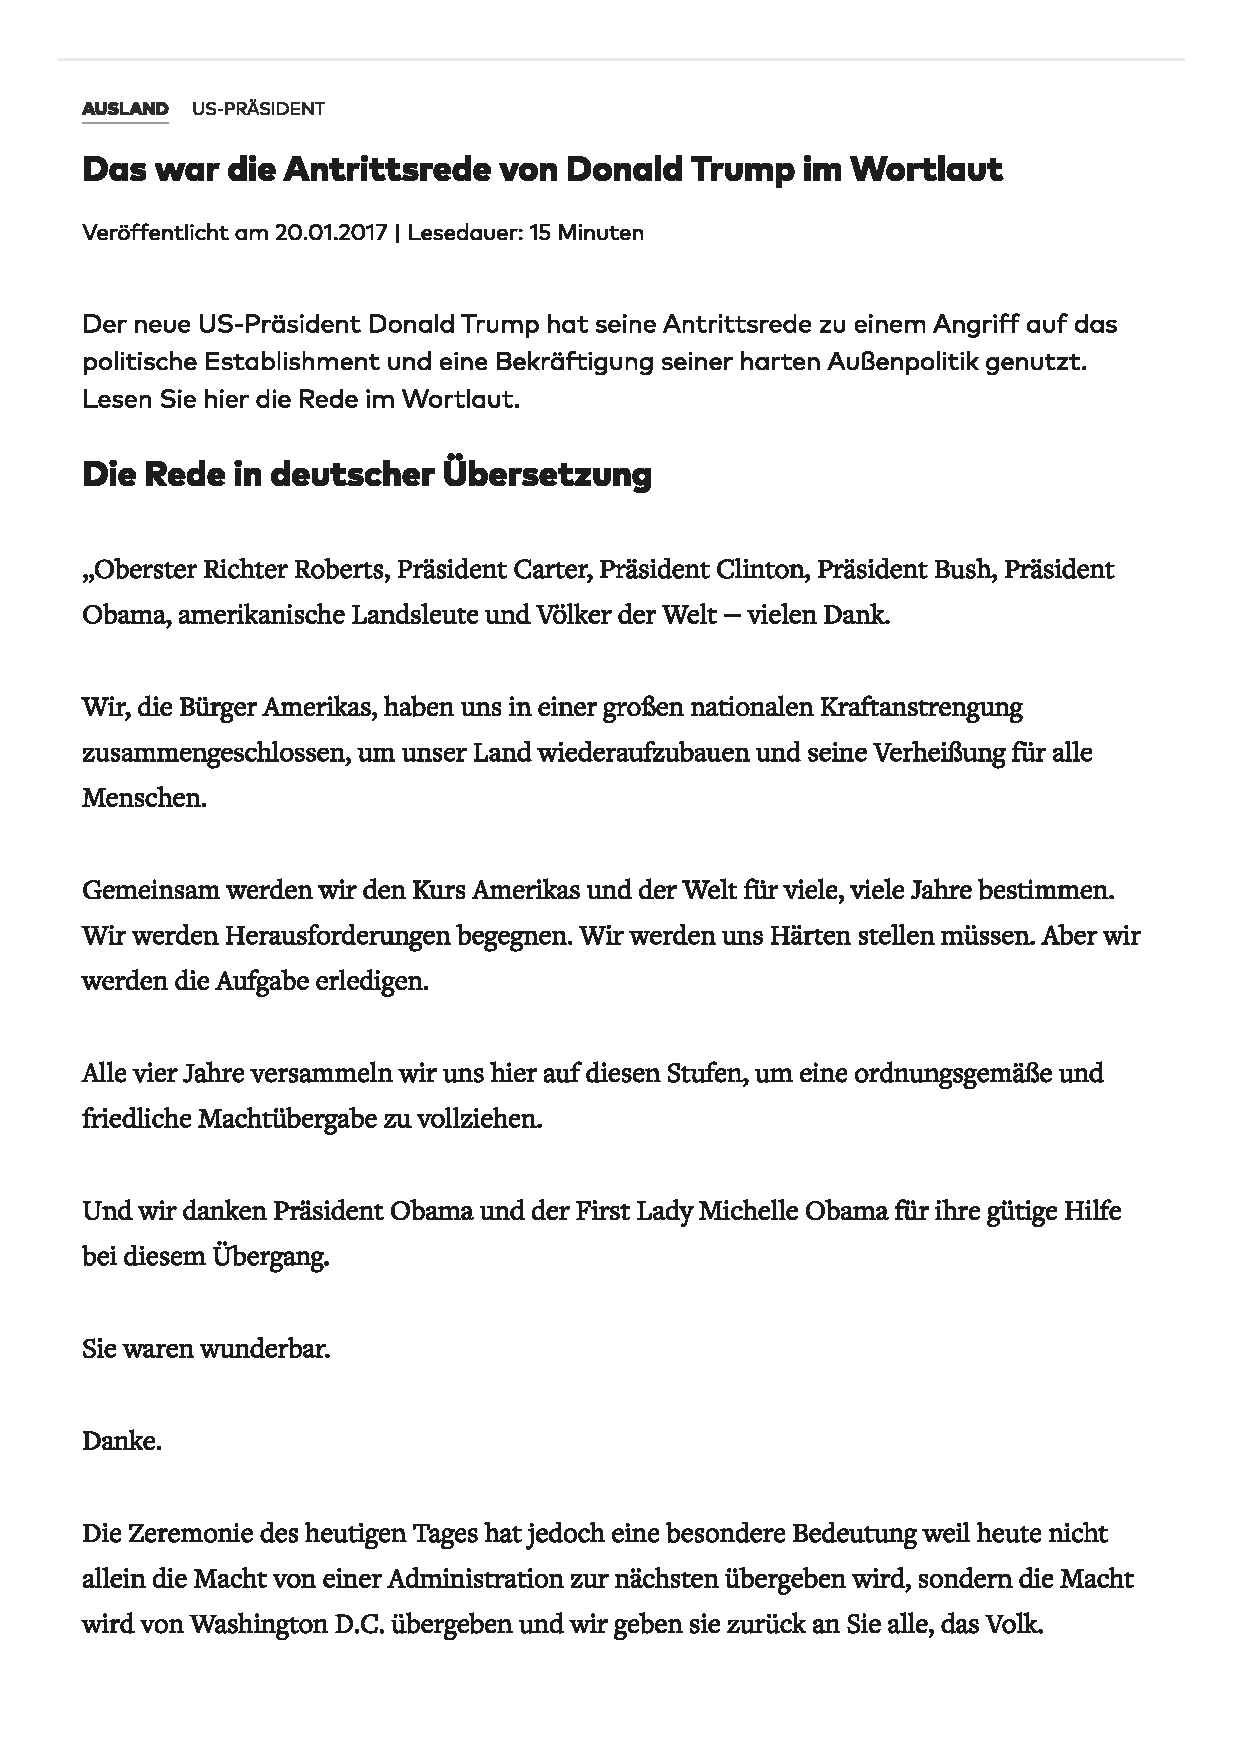
\includepdf[pages=1,scale=0.7,pagecommand={\section{Anhang}\subsection{Antrittsrede von Donald Trump}\label{ch:turing_materials}\hfill}]{Anhang/Trump_Antrittsrede_2017.pdf}
\includepdf[pages=2-,scale=.7,pagecommand={},linktodoc=true]{Anhang/Trump_Antrittsrede_2017.pdf}


\includepdf[pages=1,scale=0.7,pagecommand={\subsection{Coronarede von Angela Merkel}\label{ch:turing_materials}\hfill}]{Anhang/Merkel_Coronarede.pdf}

\includepdf[pages=2-,scale=.7,pagecommand={},linktodoc=true]{Anhang/Merkel_Coronarede.pdf}
\subsection{Begriffserklärung}
\label{sec:Begriffserklärung}
% \addcontentsline{toc}{subsection}{Begriffserklärung}
\begin{description}
  \item[linguistische Eigenschaften] - sprachliche Merkmale
  \item[Phraseologie] - Redensart einer Sprache
  \item[Paralellismen] - Wortwiederholungen
  \item[Hyperbel] - Übertreibungen
  \item[Metapher] - bildliche Sprache
  \item[dysphemistischer Ausdruck] - negativer Ausdruck/ Äußerungen
  \item[Parataxen] - unabhängige kurze Sätze
  \item[Correctivo] - Stilmittel, wenn der Redner sich selbst berichtigt
  \item[Paradoxon] - Stilmittel, mit einer wiederprüchlichen Behauptung 
  \item[Anapher] - Stilmittel, Wiederholung eines Wortes am Satzanfang 
  \item[populistische Züge] - Stimmung hervorrufen  
\end{description}
\cleardoublepage

\renewcommand{\refname}{Literaturverzeichnis}
\bibliography{Bibliographie}
\bibliographystyle{Allgemein/natdin} % DIN-Stil des Literaturverzeichnisses

\textbf{Buch-Quellen:}
\begin{itemize}
    \item Name: Rhetorik zur Eiführung, Autor: Melanie Möller (Kapitel: 2.1 und 2.4 )
    \item Name: Reden können in der Demokratie/1. Grundlagen rhetorischer Kommunikation, Autor: Joachim Detjen (Kapitel: 2.4 und 2.6)
\end{itemize}

\textbf{Internet-Quellen:}\\
\\Die 3 Säulen der Rhetorik für bewegende Landing-Page-Optimierung
\begin{itemize}
    \item Kapitel: 2.3
    \item Zugriffszeit: 28.12.2023, 14:47
    \item Link: https://blog.hubspot.de/website/landing-page-optimierung-nach-aristoteles
\end{itemize}
Ethos in Beispielsätzen
\begin{itemize}
    \item Kapitel: 2.3.1
    \item Zugriffszeit: 01.01.2024, 15:12
    \item Link: https://www.collinsdictionary.com/de/satze/deutsch/ethos
\end{itemize}
Ethos. Pathos. Logos
\begin{itemize}
    \item Kapitel: 2.3.1 und 2.3.2 
    \item Zugriffszeit: 01.01.2024, 15:34  
    \item Link: https://starkmitworten.de/ethos-pathos-logos/
\end{itemize}
Logos,Ethos und Pathos: Die drei Säulen erfolgreicher Rhetorik 
\begin{itemize}
    \item Kapitel: 2.3.2 und 2.3.3
    \item Zugriffszeit: 01.01.2024, 16:24  
    \item Link: https://bileico.com/blog/logos-ethos-pathos-rhetorik.html
\end{itemize}
Rhetorische Mittel
\begin{itemize}
    \item Kapitel: 2.4.1
    \item Zugriffszeit: 02.01.2024, 18:30
    \item Link: https://www.stagement.com/blog/rede-verbessern-rhetorischestilmittel/
\end{itemize}
Rhetorische Mittel Definition, Liste und Beispiele
\begin{itemize}
    \item Kapitel: 2.4
    \item Zugriffszeit: 02.01.2024, 18:54
    \item Link: https://www.bachelorprint.de/wissenschaftliches-schreiben/rhetorische-mittel/ 
\end{itemize}
Rhetorische Mittel: Bedeutung und Beispiele
\begin{itemize}
    \item Kapitel: 2.4
    \item Zugriffszeit: 02.01.2024, 21:52  
    \item Link: https://lessons2go.de/magazin/artikel/rhetorische-mittel-bedeutung-beispiele.html
\end{itemize}
Rhetorische Mittel Liste mit Beispielen und Erklärungen
\begin{itemize}
    \item Kapitel: 2.4
    \item Zugriffszeit: 02.01.2024, 22:17 
    \item Link: https://www.scribbr.de/wissenschaftliches-schreiben/rhetorische-mittel/    
\end{itemize}
Rhetorik im Alltag und Beruf: Warum es sich lohnt, Ihre Fähigkeiten zu verbessern
\begin{itemize}
    \item Kapitel: 2.5
    \item Zugriffszeit: 03.01.2024 14:59  
    \item Link: https://www.openpr.de/news/1244738/Rhetorik-im-Alltag-und-Beruf-Warum-es-sich-lohnt-Ihre-Faehigkeiten-zu-verbessern.html.   
\end{itemize}
Rhetorik: Diese 8 Fehler solltest du vermeiden, um kraftvoll zu kommunizieren
\begin{itemize}
    \item Kapitel: 2.5
    \item Zugriffszeit: 07.01.2024, 17:32  
    \item Link: https://www.stellenanzeigen.de/careeasy/kraftvoll-kommunizieren-sde18286/   
\end{itemize}
Rhetorik Definition
\begin{itemize}
    \item Kapitel: 2.6
    \item Zugriffszeit: 20.02.2024, 16:59  
    \item Link: https://www.rhetorik-homepage.de/
\end{itemize}
Rhetorik für den Alltag
\begin{itemize}
    \item Kapitel: 2.5 und 2.6 
    \item Zugriffszeit: 03.01.2024, 15:27   
    \item Link: https://www.rheacting.de/rhetorik-fuer-den-alltag/  
\end{itemize}
% !TEX root = Projektdokumentation.tex
\clearpage
\addsec{Eidesstattliche Erklärung}

% Hinweis: die eidesstattliche Erklärung ist ggfs. an die Richtlinie der IHK anzupassen

Ich, \autorName, versichere hiermit, dass ich meine \textbf{\betreff} mit dem
Thema
\begin{quote}
\textit{\kompletterTitel}
\end{quote}
selbständig verfasst und keine anderen als die angegebenen Quellen und Hilfsmittel benutzt habe,
wobei ich alle wörtlichen und sinngemäßen Zitate als solche gekennzeichnet habe. Die Arbeit
wurde bisher keiner anderen Prüfungsbehörde vorgelegt und auch nicht veröffentlicht.\\[6ex]

\abgabeOrt, den \abgabeTermin


\rule[-0.2cm]{5.5cm}{0.5pt}

\textsc{\autorName}

\cleardoublepage

% \subsection{Antrittsrede von Donald Trump}
% \label{sec: Trumps Rede}
% 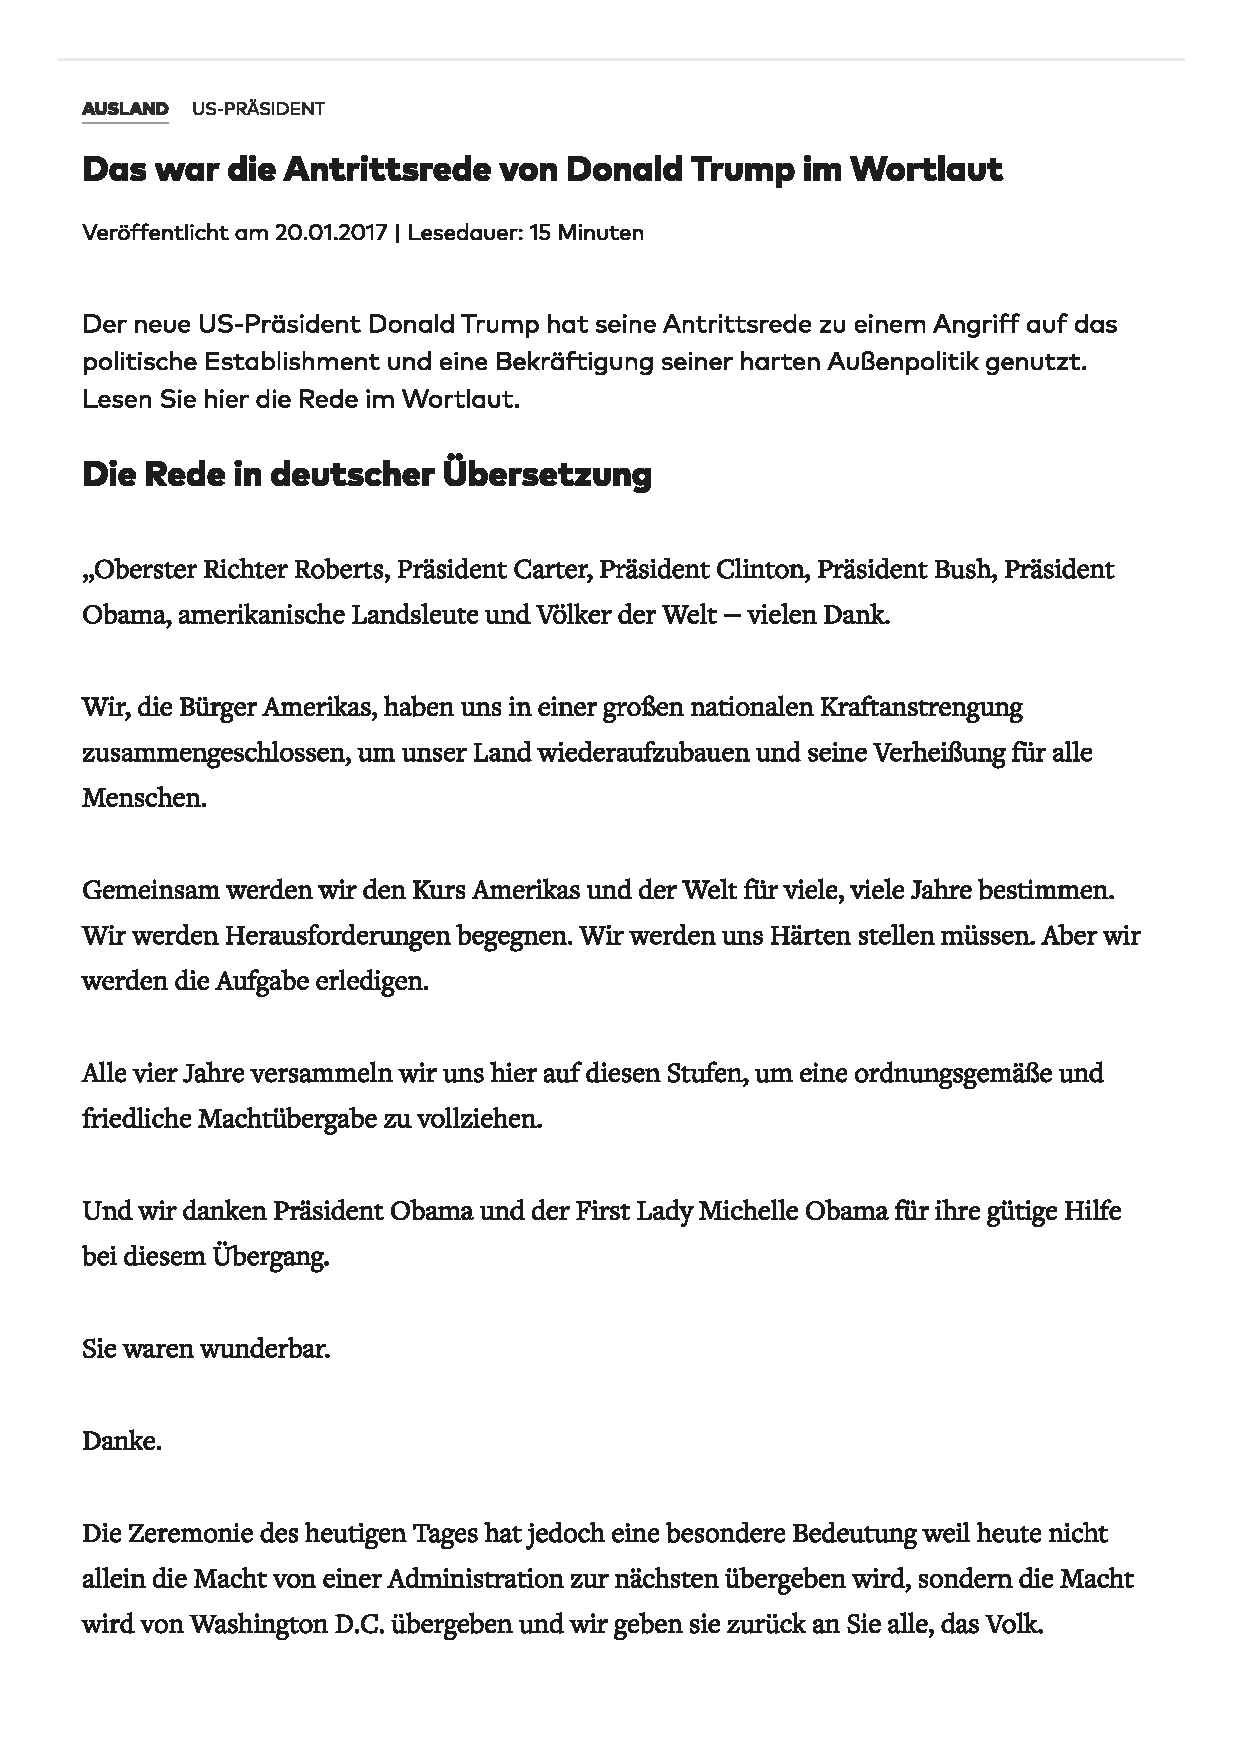
\includepdf[pages=1-11]{Anhang/Trump_Antrittsrede_2017.pdf}

% \subsection{Rede von Angela Merkel}
% \label{sec: Rede von Merkel}
% 
\includepdf[pages=1-7]{Anhang/Merkel_Coronarede.pdf}